% Created 2020-03-26 Thu 18:01
% Intended LaTeX compiler: pdflatex
\documentclass[11pt]{article}
\usepackage[utf8x]{inputenc}
\usepackage[T1]{fontenc}
\usepackage{graphicx}
\usepackage{grffile}
\usepackage{longtable}
\usepackage{wrapfig}
\usepackage{rotating}
\usepackage[normalem]{ulem}
\usepackage{amsmath}
\usepackage{textcomp}
\usepackage{amssymb}
\usepackage{capt-of}
\usepackage{hyperref}
\usepackage{minted}
\usepackage[margin=1in]{geometry}
\author{Jakub Zárybnický}
\date{25. března 2020}
\title{Implementace algoritmu "Odd-even~transposition~sort"}
\hypersetup{
 pdfauthor={Jakub Zárybnický},
 pdftitle={Implementace algoritmu "Odd-even~transposition~sort"},
 pdfkeywords={},
 pdfsubject={},
 pdfcreator={Emacs 26.3 (Org mode 9.1.9)}, 
 pdflang={English}}
\begin{document}

\maketitle

\section{Algoritmus}
\label{sec:orgfc8b5dd}
Algoritmus pracuje s lineárně propojenou sadou procesorů, pro uspořádání N
hodnot použijeme N procesorů, kde hodnoty jsou distribuované v přípravném kroku
algoritmu.

Pokud se v jednom kroku přesune jedna hodnota nejvýše o jeden procesor doleva či
doprava, potřebujeme právě N kroků pro seřazení opačně uspořádané sekvence -
tj. pro přesunutí nejmenší hodnoty např. z pravého konce doleva. Pokud nazveme
jednotlivé kroky algoritmu "distribute", "sort" a "collect", pak
\begin{enumerate}
\item "distribute" je v odevzdané implementaci \(O(n)\), odesíláme hodnoty po
jedné. Při využití sdílené paměti by ale krok "distribute" mohl mít \(O(1)\),
kdy každý procesor by si načetl svou hodnotu z paměti v jednom kroku;
\item "sort" je jádro algoritmu. Za použití lineární topologie a \(N\) procesorů pro
\(N\) hodnot je nutný počet kroků lineární, \(O(N)\), za předpokladu opačně
seřazené sekvence;
\item "collect" má stejně jako "distribute" časovou složitost \(O(n)\), nejlevější
procesor přijímá hodnoty po jedné. Za použití sdílené paměti by ale
složitost mohla být \(O(1)\).
\end{enumerate}

Celková časová složitost je tedy lineární, \(t(n) = O(n)\). Celková prostorová
složitost je také lineární, n procesorů (s jedním paměťovým slotem), \(p(n) =
O(n) = O(n)\). Celková cena algoritmu je ale \(c(n) = t(n) * p(n) = O(n^2)\),
kdežto optimální složitost pro algoritmus paralelního řazení je \(O(log n)\).

\section{Implementace}
\label{sec:org6243153}
Implementovaný program také pracuje ve třech krocích, ve fázi "distribute" se
načtou data ze souboru v procesu s rankem 0 a pomocí primitivní operace
\texttt{MPI\_Scatter} se jednotlivé položky dostanou i k ostatním procesům.

Fáze "sort" probíhá různě pro sudé/liché procesy, kdy v sudých cyklech dostanou
sudé procesy hodnotu svého levého souseda a rozhodnou se, jestli transponovat
nebo ne (kombinace operací \texttt{MPI\_Send} a \texttt{MPI\_Recv}), v lichých cyklech toto
provádějí zase procesy liché.

V závěrečné fázi "collect" se pro sesbírání dat od jednotlivých procesů použije
\texttt{MPI\_Gather}, a proces s rankem 0 vypíše už uspořádaná data.

\section{Experimenty}
\label{sec:org4bcccb7}
\begin{center}
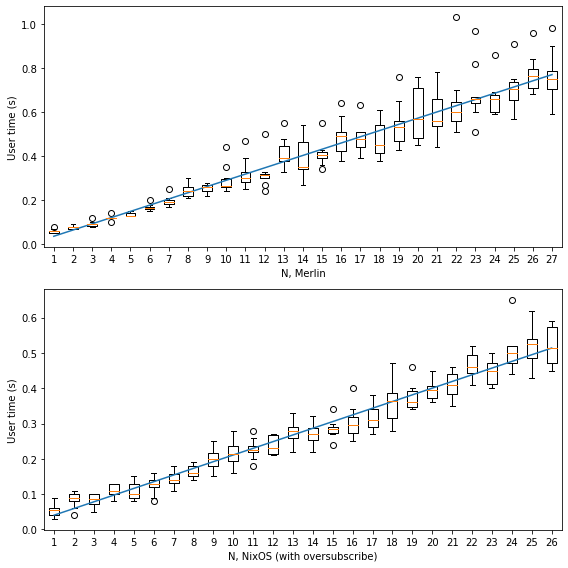
\includegraphics[width=.9\linewidth]{./.ob-jupyter/10773b02fdc9c6bbbe7ad2653184b22029124297.png}
\end{center}

Experimenty byly provedeny pomocí shell skriptu, ve kterém bylo pro N z
intervalu od 1 do 26, resp. 27 pro Merlina, provedeno deset měření pomocí
příkazu \texttt{time} (\texttt{/usr/bin/time}, ne vestavěný příkaz terminálu). Pro každé měření
byla vygenerována nová sada N vstupních hodnot spuštěn program pomocí \texttt{mpirun},
měřena byla celková doba běhu příkazu \texttt{mpirun}. Výstupem tohoto skriptu byl CSV
soubor s jednotlivými naměřenými hodnotami (parametr N, \texttt{wall time}, \texttt{user time},
\texttt{kernel time}).

Měření jsem provedl na Merlinovi a na svém osobním počítači (za použití
\texttt{-{}-oversubscribe}), pro vytvoření grafu jsem použil sloupec \texttt{user time} a knihovnu
\texttt{matplotlib}. Z těchto hodnot je zakreslen výše přiložený boxplot (za použití
výchozího nastavení), včetně regresní přímky proložené získanými hodnotami.

\section{Protokol}
\label{sec:orgdb8d12e}
\begin{center}
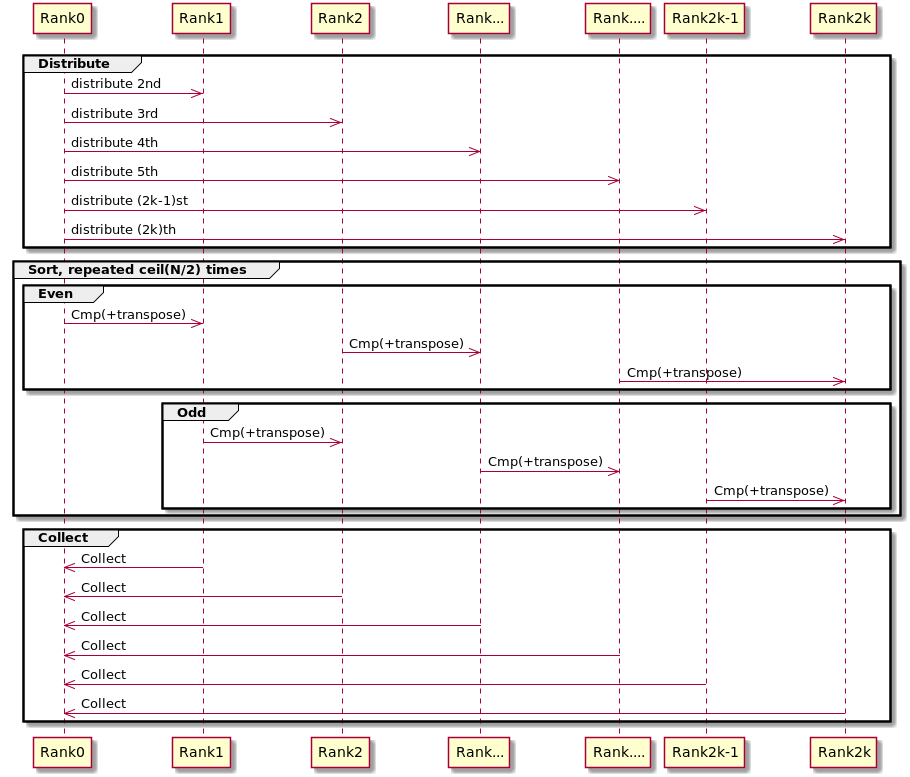
\includegraphics[width=.9\linewidth]{odd-even.png}
\end{center}

\section{Závěr}
\label{sec:orgf770d37}
Z výsledného grafu experimentu je zřejmé, že lineární časová náročnost
implementovaného algoritmu odpovídá teoretické časové složitosti. Počet hodnot
\emph{outliers} naměřených na Merlinovi je sice nečekaně mnoho, předpokládám ale, že to
bylo způsobené procesy jiných uživatelů, při dalších měřeních se stejný problém
už neopakoval.

Absolutní časové hodnoty, např. 0.8s pro seřazení 27 čísel na merlinovi, jsou
sice pro program s touto funkčností nepřijatelné - nejen algoritmus není
optimální svou celkovou cenou jakožto algoritmus pro paralelní řazení, ale
implementační volba OpenMPI způsobuje, že čas potřebný pro režii komunikace mezi
procesy zcela dominuje času spotřebovaný pro řazení samotné.
\end{document}